%\documentclass[tikz,convert={outfile=\jobname.svg}]{standalone}
\documentclass[tikz]{standalone}
%\documentclass{article}
%\documentclass[crop,tikz,convert={outext=.svg,command=\unexpanded{pdf2svg \infile\space\outfile}},multi=false]{standalone}[2012/04/13]
%\usetikzlibrary{...}% tikz package already loaded by 'tikz' option
%\makeatletter

%\usepackage[paperheight=4in,paperwidth=4in,margin=0in]{geometry}

%\usepackage{tikz} % already loaded
\usetikzlibrary{bayesnet}
\usetikzlibrary{shapes.geometric} % needed for squares

\usepackage{graphics}
%\pgfrealjobname{survey}
%pdflatex --jobname=ordinalModel1 graphicalModels.tex

\newcommand{\Irater}{r}
\newcommand{\Iitem}{i}
\newcommand{\Ipatient}{p}
\newcommand{\Incat}{c}
\newcommand{\Ilatent}{l}

\newcommand{\Trater}{\expandafter\MakeUppercase\expandafter{\Irater}}
\newcommand{\Titem}{\expandafter\MakeUppercase\expandafter{\Iitem}}
\newcommand{\Tpatient}{\expandafter\MakeUppercase\expandafter{\Ipatient}}
\newcommand{\Tncat}{\expandafter\MakeUppercase\expandafter{\Incat}}
\newcommand{\Tlatent}{\expandafter\MakeUppercase\expandafter{\Ilatent}}

\tikzstyle{obsD} = [square,fill=gray!25,draw=black,inner sep=1pt,minimum size=20pt, font=\fontsize{10}{10}\selectfont, node distance=1]
\tikzstyle{obsC} = [circle,fill=gray!25,draw=black,inner sep=1pt,minimum size=20pt, font=\fontsize{10}{10}\selectfont, node distance=1]

\begin{document}
	
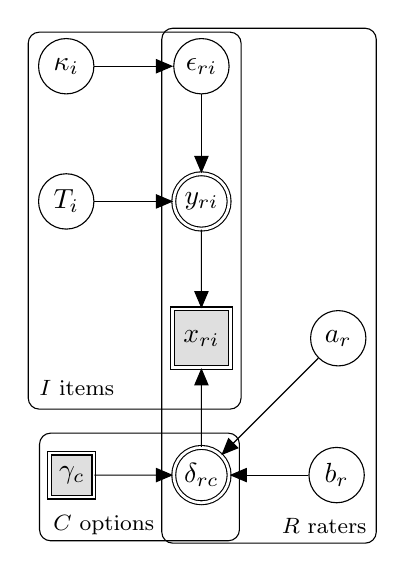
\begin{tikzpicture}[square/.style={regular polygon,regular polygon sides=4}]
%\draw [help lines] (-3,-5) grid (3,5);			

% Define nodes
\node[obsD, double distance=1pt]                        (x) {$x_{\Irater\Iitem}$};
\node[latent, below = of x, double distance = 1pt]      (d) {$\delta_{\Irater\Incat}$};
\node[latent, right = of x]                             (a) {$a_\Irater$};
\node[latent, right = of d]                             (b) {$b_\Irater$};
\node[obsD, left  = of d, double distance = 1pt]        (g) {$\gamma_\Incat$};

\node[latent, above = of x, double distance = 1pt]      (y) {$y_{\Irater\Iitem}$};
\node[latent, above = of y]                             (e) {$\epsilon_{\Irater\Iitem}$};
\node[latent, left  = of y]                             (t) {$T_\Iitem$};
%\node[latent, right = of e] 						    (E) {$\zeta_\Irater$};
\node[latent, right = of e, draw = none] 				(E) {};
\node[latent, left  = of e] 						    (tau) {$\kappa_\Iitem$};

% Edges
\edge {d}       {x};%
\edge {a, b, g} {d};%
\edge {t, e}    {y};%
\edge {y}       {x};%
%\edge {E}       {e};%
\edge {tau}     {e};%

\plate[text centered] {ni} {(a)(b)(d)(x)(y)(e)(E)}     {$\Trater$ raters };
{\tikzset{plate caption/.append style={below=4pt of #1.south west, xshift = .5cm}}
\plate[text centered, yshift = -.05cm] {ni} {(t)(x)(y)(e)(tau)}            {$\Titem$ items  };
}
{\tikzset{plate caption/.append style={below=4pt of #1.south west, xshift = .7cm}}
\plate[text centered, yshift =  .05cm] {nc} {(g)(d)}              {$\Tncat$ options};
}

\end{tikzpicture}

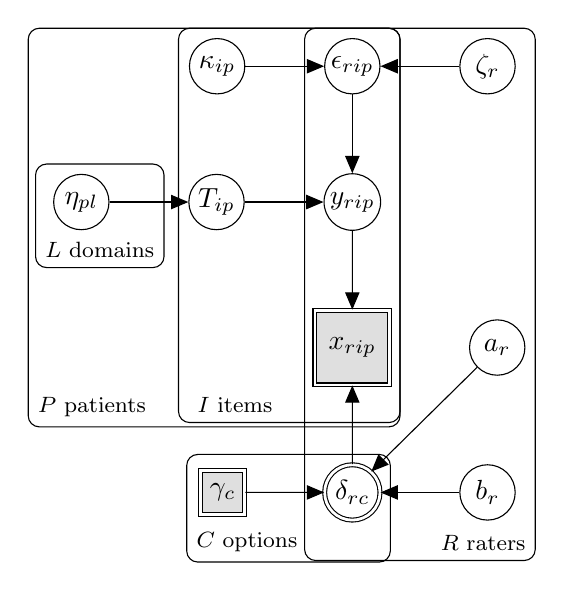
\begin{tikzpicture}[square/.style={regular polygon,regular polygon sides=4}]
%\draw [help lines] (-3,-5) grid (3,5);			

% Define nodes
\node[obsD, double distance=1pt]                        (x) {$x_{\Irater\Iitem\Ipatient}$};
\node[latent, below = of x, double distance = 1pt]      (d) {$\delta_{\Irater\Incat}$};
\node[latent, right = of x]                             (a) {$a_\Irater$};
\node[latent, right = of d]                             (b) {$b_\Irater$};
\node[obsD, left  = of d, double distance = 1pt]        (g) {$\gamma_\Incat$};

\node[latent, above = of x]                             (y) {$y_{\Irater\Iitem\Ipatient}$};
\node[latent, above = of y]                             (e) {$\epsilon_{\Irater\Iitem\Ipatient}$};
\node[latent, left  = of y]                             (t) {$T_{\Iitem\Ipatient}$};

\node[latent, right = of e] 						    (E) {$\zeta_\Irater$};
\node[latent, left  = of e] 						    (tau) {$\kappa_{\Iitem\Ipatient}$};

\node[latent, left  = of t] 						    (l) {$\eta_{\Ipatient\Ilatent}$};

% Edges
\edge {d}       {x};%
\edge {a, b, g} {d};%
\edge {t, e}    {y};%
\edge {y}       {x};%
\edge {E}       {e};%
\edge {tau}     {e};%
\edge {l}       {t};%

\plate[text centered] {ni} {(a)(b)(d)(x)(y)(e)(E)}     {$\Trater$ raters };
{\tikzset{plate caption/.append style={below=4pt of #1.south west, xshift = .6cm}}
	\plate[text centered] {ni} {(t)(x)(y)(e)(tau)}            {$\Titem$ items  };
}
{\tikzset{plate caption/.append style={below=4pt of #1.south west, xshift = .6cm}}
	\plate[text centered] {nc} {(g)(d)}              {$\Tncat$ options};
}
{\tikzset{plate caption/.append style={below=4pt of #1.south west, xshift = .5cm}}
	\plate[text centered] {ni} {(t)(x)(y)(e)(l)}            {$\Tpatient$ patients  };
}
{\tikzset{plate caption/.append style={below=4pt of #1.south west, xshift = .6cm}}
	\plate[text centered] {ni} {(l)}     {$\Tlatent$ domains };
}
\end{tikzpicture}

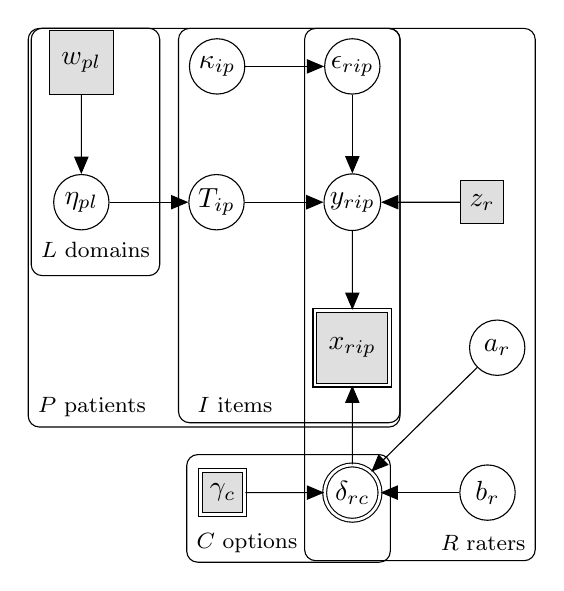
\begin{tikzpicture}[square/.style={regular polygon,regular polygon sides=4}]
%\draw [help lines] (-3,-5) grid (3,5);			

% Define nodes
\node[obsD, double distance=1pt]                         (x) {$x_{\Irater\Iitem\Ipatient}$};
\node[latent, below = of x, double distance = 1pt]      (d) {$\delta_{\Irater\Incat}$};
\node[latent, right = of x]                             (a) {$a_\Irater$};
\node[latent, right = of d]                             (b) {$b_\Irater$};
\node[obsD, left  = of d, double distance = 1pt]        (g) {$\gamma_\Incat$};

\node[latent, above = of x]                             (y) {$y_{\Irater\Iitem\Ipatient}$};
\node[latent, above = of y]                             (e) {$\epsilon_{\Irater\Iitem\Ipatient}$};
\node[latent, left  = of y]                             (t) {$T_{\Iitem\Ipatient}$};

%\node[latent, right = of e] 						    (E) {$\zeta_\Irater$};
\node[latent, right = of e, draw = none] 				(E) {};
\node[latent, left  = of e] 						    (tau) {$\kappa_{\Iitem\Ipatient}$};

\node[latent, left  = of t] 						    (l) {$\eta_{\Ipatient\Ilatent}$};

\node[obsD,    right = of y] 						    (z)  {$z_{\Irater}$};
\node[obsD,   above = of l]  						    (w) {$w_{\Ipatient\Ilatent}$};


% Edges
\edge {d}       {x};%
\edge {a, b, g} {d};%
\edge {t, e, z} {y};%
\edge {y}       {x};%
%\edge {E}       {e};%
\edge {tau}     {e};%
\edge {l}       {t};%
\edge {w}       {l};%

\plate[text centered] {ni} {(a)(b)(d)(x)(y)(e)(E)}     {$\Trater$ raters };
{\tikzset{plate caption/.append style={below=4pt of #1.south west, xshift = .6cm}}
	\plate[text centered] {ni} {(t)(x)(y)(e)(tau)}            {$\Titem$ items  };
}
{\tikzset{plate caption/.append style={below=4pt of #1.south west, xshift = .6cm}}
	\plate[text centered] {nc} {(g)(d)}              {$\Tncat$ options};
}
{\tikzset{plate caption/.append style={below=4pt of #1.south west, xshift = .5cm}}
	\plate[text centered] {ni} {(t)(x)(y)(e)(l)}            {$\Tpatient$ patients  };
}
{\tikzset{plate caption/.append style={below=4pt of #1.south west, xshift = .6cm,yshift=0cm}}
	\plate[text centered, yshift = -.1cm] {ni} {(l)(w)}     {$\Tlatent$ domains };
}
\end{tikzpicture}

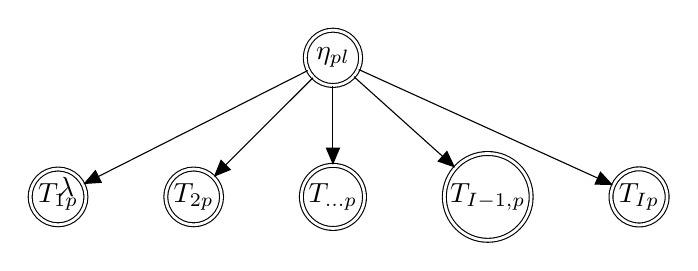
\begin{tikzpicture}[square/.style={regular polygon,regular polygon sides=4}]
%\draw [help lines] (-3,-5) grid (3,5);			

\node[latent, double distance = 1pt]                      (lt1) {$T_{1\Ipatient}$};
\node[latent, right = of lt1, double distance = 1pt]      (lt2) {$T_{2\Ipatient}$};
\node[latent, right = of lt2, double distance = 1pt]      (lt3) {$T_{\dots\Ipatient}$};
\node[latent, right = of lt3, double distance = 1pt]      (lt4) {$T_{\Titem-1, \Ipatient}$};
\node[latent, right = of lt4, double distance = 1pt]      (lt5) {$T_{\Titem\Ipatient}$};

\node[latent, above = of lt3, double distance = 1pt]      (eta) {$\eta_{\Ipatient\Ilatent}$};

% Edges
\edge {eta}       {lt1, lt2, lt3, lt4, lt5} {$\lambda$};%
\end{tikzpicture}


\end{document}


